% Folien f�r die Poster-Session VAR2021
\documentclass[aspectratio=169]{beamer}
% Funktion f�r Footer/Header in den Folien
\newcommand{\lectureName}{Visual Raytrace}
% Titel der Folie
\title{\lectureName}
\author{Manfred Brill, Benedict S�rota}
\institute{University of Applied Sciences Kaiserslautern}
\date[]{}
%
% Variablen wie Semester ...
%
\newcommand{\theSemester}{September 2021}
% Standardverzeichnis f�r das Basis-Verzeichnis der Bilder
%
\newcommand{\imagePath}{../figures}
%
% Name der Bilddatei, die auf die Fragefolie kommen soll
\newcommand{\questionImage}{../figures/vorgang}

\input{slidesheader}
\title{Visual$\:$Raytrace}
\subtitle{VAR 2021 --- Poster Session}
%
%
\subject{Informatik -- Masterstudiengang}
\keywords{Informatik, Masterstudiengang, Master of Science, Hochschule Kaiserslautern, Fachbereich Informatik und Mikrosystemtechnik}
%
\hypersetup{
pdfauthor = {Manfred Brill, Benedict Särota},
pdfsubject = {Poster Visual Raytrace VAR2021},
pdftitle = {MasterstPoster Visual Raytrace VAR2021},
pdfkeywords = {Immersive Learning, Computer Graphics, Raytracing, VR, XR, University of Applied Sciences Kaiserslautern, Computer Science},
pdfpagelayout = SinglePage,
pdfpagemode = UseThumbs,
pdfdisplaydoctitle = true
}

%
\setboolean{solutions}{true}
% Nur Folien: die n�chste Zeile kommentieren!
\setbeameroption{show notes}
% Die n�chste Zeile dekommentieren f�r handouts!
\pgfpagesuselayout{2 on 1}[a4paper, border shrink=5mm]
%
\begin{document}
\begin{frame}
  \titlepage
  \begin{center}
   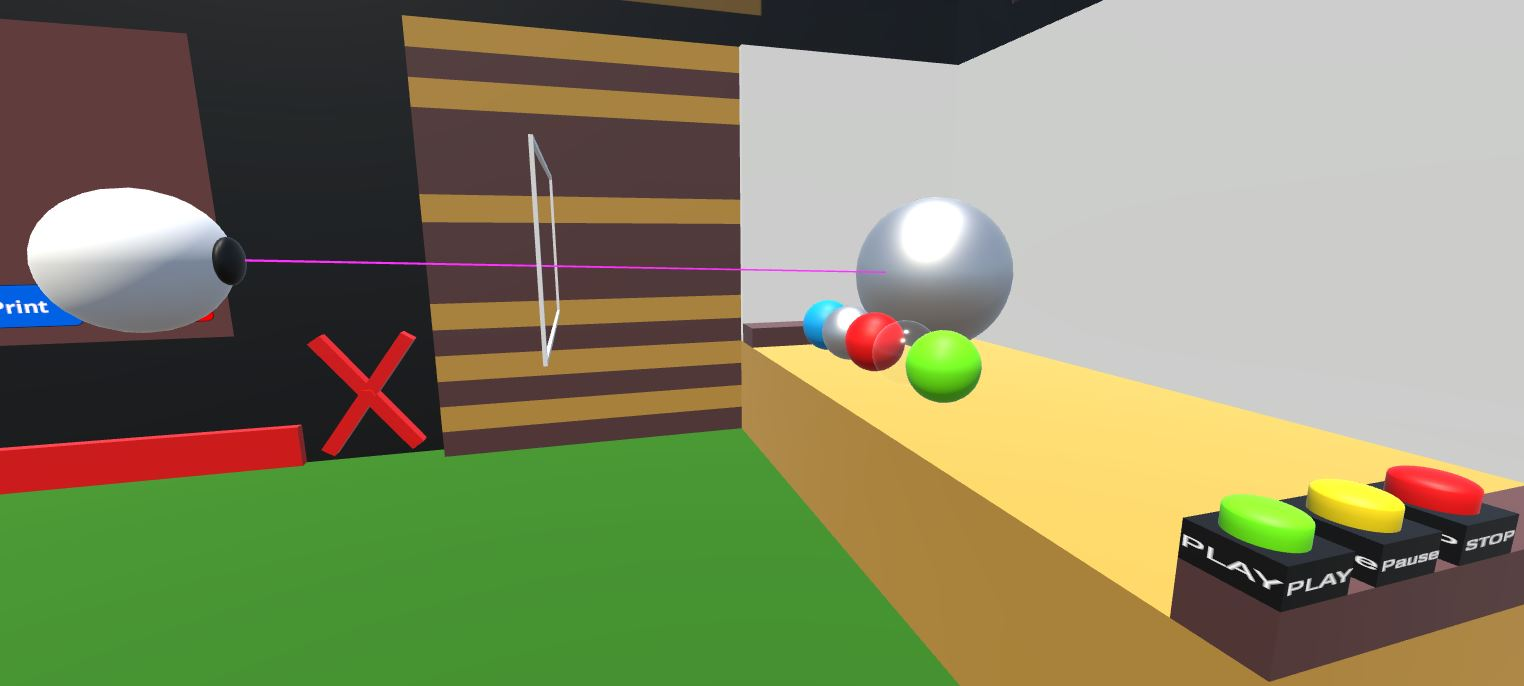
\includegraphics[width = 5.0cm]{\imagePath/vorgang}
  \end{center}
\end{frame}

\note{
\noteshead{Information}

\begin{description}
\item[Thema:]  Folien f�r die Poster-Session auf der VAR 2021
\item[Version:] \theSemester{}
\item[Dateiname:] postersession.tex
\end{description}

Folien werden mit \lstinline$\\begin\{frame\}$ \ldots \lstinline$\\end\{frame\}$ eingef�gt.

Die Vorlagen verwenden die Datei slidesheader.tex, die man auf Styles and More auf Github findet!
}

\section{Motivation}
\note{
\noteshead{Notes}

Hier k�nnen wir Notizen schreiben, die wir in den Handouts auch ausdrucken k�nnen!

Als erster Schritt wurden einfach die Bilder und Texte aus dem Poster �bernommen.
F�r Folien, die nur eine �berschrift und ein Bild verwenden gibt es in slidesheader.tex
die Funktion \lstinline$\\imageslide$. Erstes Argument ist der Titel, dann die Angabe der Breite (am Besten
in Prozent der Textbreite) und den Pfad f�r das Bild (relativ zum Inhalt
der Variablen \lstinline$\\imagePath$.
}

\note{
\noteshead{Textblock}

Die folgende Folie verwendet den Textblock aus dem Poster oben rechts!
}

\begin{frame}{Immersive Learning}
\begin{block}{Raytracing}
   \begin{itemize}
   \item Raytracing is one of the major topics in computer graphics classes.
   \item Students have to implement their own version of a working raytracer.
   \item To implement a raytracer students need to understand the basic concepts of computer graphics
   like coordinate systems, camera, lighting or reflection.
   \item Key for the successful implementation of a raytracer by the students: develop a high spatial imagination.
   \item The immersive learning application \textbf{Visual$\:$Raytrace} supports the transfer from 3D space
   to a programming language and deepens the understanding of the basic concepts of a raytracer.
   \end{itemize}
\end{block}
\end{frame}

\note{
\noteshead{Bilder aus dem Poster}

Hier wurden jetzt einfach die Bilder aus dem Poster eingebaut.

Mit \lstinline$\\section$ wird links oben die �berschrift eingestellt (kann man auch leer lassen.

Das rechte Feld k�nnen wir auch ausf�llen, mit \lstinline$\\subsection$.
}

\section{Whitted Raytracing}
\imageslide{Whitted Raytracing}{0.7\textwidth}{whitted02}

\section{Visual$\:$Raytrace}
\imageslide{A Raytracer in a Virtual Environment}{0.9\textwidth}{duringProcess}

\imageslide{A Virtual Framebuffer and a Virtual Ray}{0.9\textwidth}{duringProcessEyeView}

\imageslide{Ray-Sphere Intersection}{0.9\textwidth}{duringProcessHitObjects}

\imageslide{Interactive Scene Definition}{0.9\textwidth}{sphereCreating}

\imageslide{Settings for the Raytracer}{0.9\textwidth}{settings}

\section{Software Development}
\imageslide{Unity and C\#}{0.9\textwidth}{unityIDE}

\questionsEnglish[0.9\textwidth]
\end{document}
